\section{推理阶段性能剖析}\label{sec:inference}

本节专门分析 SO-101 在线控制循环中的 ACT 推理阶段。
这里的“推理阶段”并不只是一次 ACT 前向计算，
而是从动作预测接口收到 observation 开始，
经过动作缓存判断、必要时的观测预处理、ACT 模型前向、动作队列写入、
再到动作反归一化返回的完整路径。

当前实验配置中，ACT 的 chunk\_size 与动作步数配置均为 100，单次完整模型推理输出
\((B,\mathrm{chunk\_size},\mathrm{action\_dim})=(1,100,6)\) 的动作序列。
因此在线循环的大多数帧并不会重新执行模型前向，而是直接从
动作队列中取出上一次推理缓存的下一帧动作。
这一区别是理解第~\ref{sec:inference} 节所有时间数据的前提：
chunk\_size 主要是在时间上分摊单次 ACT 前向开销，
而不是让一次 ACT 前向本身变快。

\subsection{动作选择接口与动作队列}

LeRobot 在动作预测接口外层先检查策略对象的动作队列。
如果动作队列非空，主循环直接取出缓存动作，再通过后处理器
反归一化为真实舵机目标；这一帧会跳过图像 tensor 转换、
预处理器和 ACT 前向计算。
只有当队列为空时，系统才会走完整推理路径：
把 numpy observation 转为 PyTorch Tensor，执行归一化预处理，
调用策略动作选择接口，继而触发动作块预测和 ACT 前向计算。
模型一次产生 100 帧归一化动作，写入队列后立即弹出第 0 帧返回；
后续 99 帧由队列快速路径逐帧取用。
动作队列快速路径与队列为空时的完整推理路径如图~\ref{fig:act-select-action-queue}所示。

\begin{figure}[htbp]
  \centering
  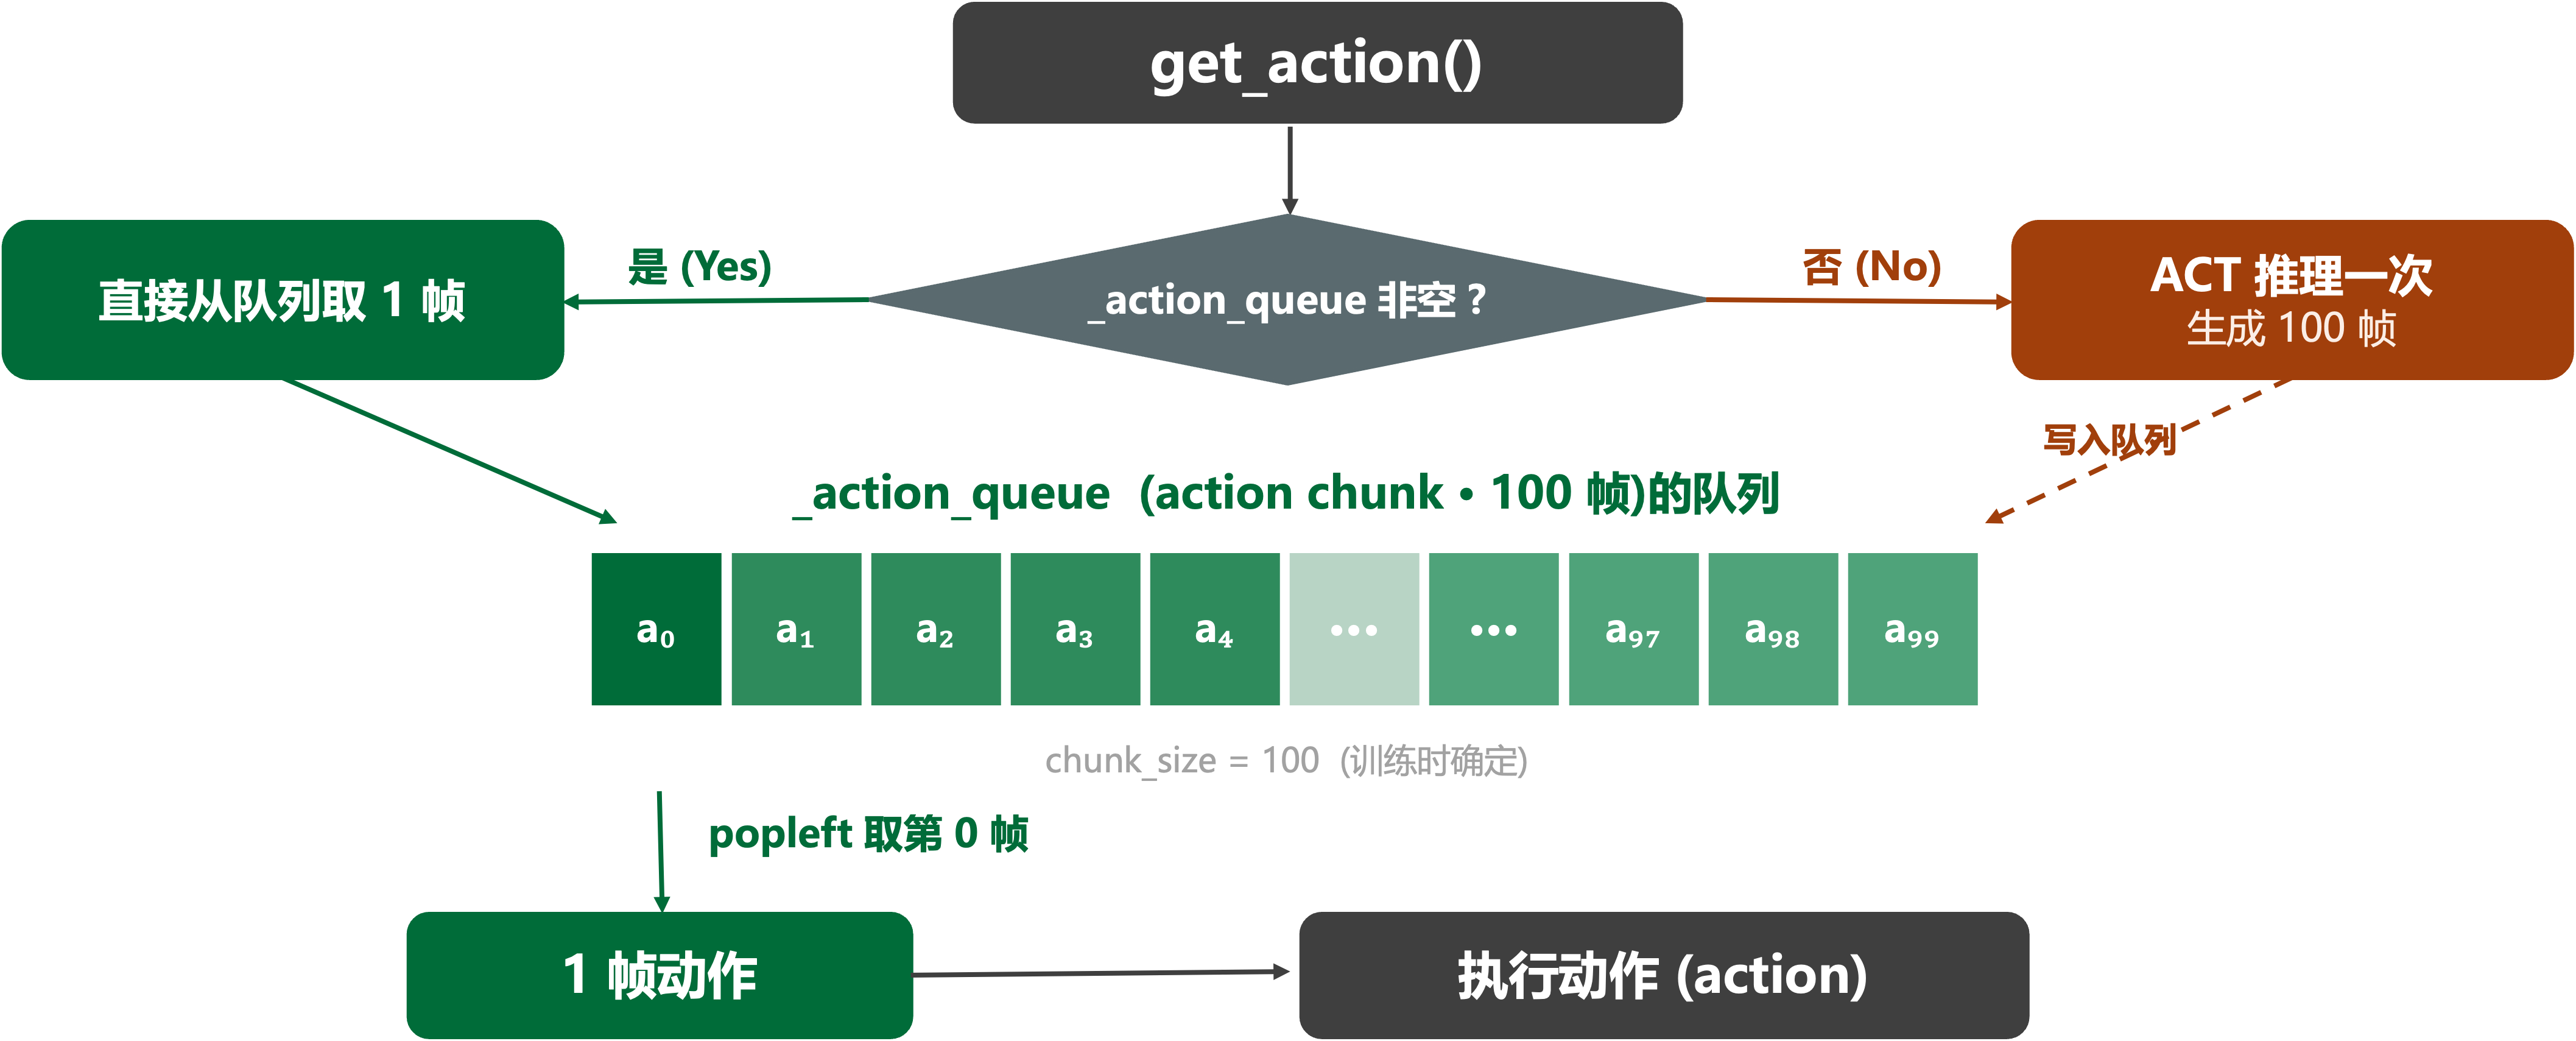
\includegraphics[width=\textwidth]{3_性能分析/image/act_select_action_queue.png}
  \caption{ACT 在线推理中动作队列快速路径与完整推理路径}
  \label{fig:act-select-action-queue}
\end{figure}

该调用路径说明了 chunk\_size 为 100 时的两种时间尺度：
队列非空帧只承担动作取队列和反归一化，属于轻量路径；
队列为空帧才承担完整 ACT 前向，属于重推理路径。
因此，按 episode 统计得到的 inference 占比，本质上是少数重推理帧
在 100 帧执行周期内被均摊后的结果。

\subsection{一次完整 ACT 推理的数据流}

队列为空时，动作预测接口会先把原始 observation
整理成 ACT 可接受的 batch。两路相机图像从
\((H,W,C)\) 的 uint8 numpy 数组转换为
\((1,3,360,640)\) 的 float32 Tensor；
关节状态从 \((6,)\) 转为 \((1,6)\)。
随后预处理器使用随 checkpoint 保存的训练集
mean/std 对图像、state 进行归一化。进入 ACT 前向计算
后，推理态下不运行训练用 VAE encoder，而是使用全零 latent。
队列为空时一次完整 ACT 推理的数据流与模型结构如图~\ref{fig:act-forward-dataflow}所示。

\begin{figure}[htbp]
  \centering
  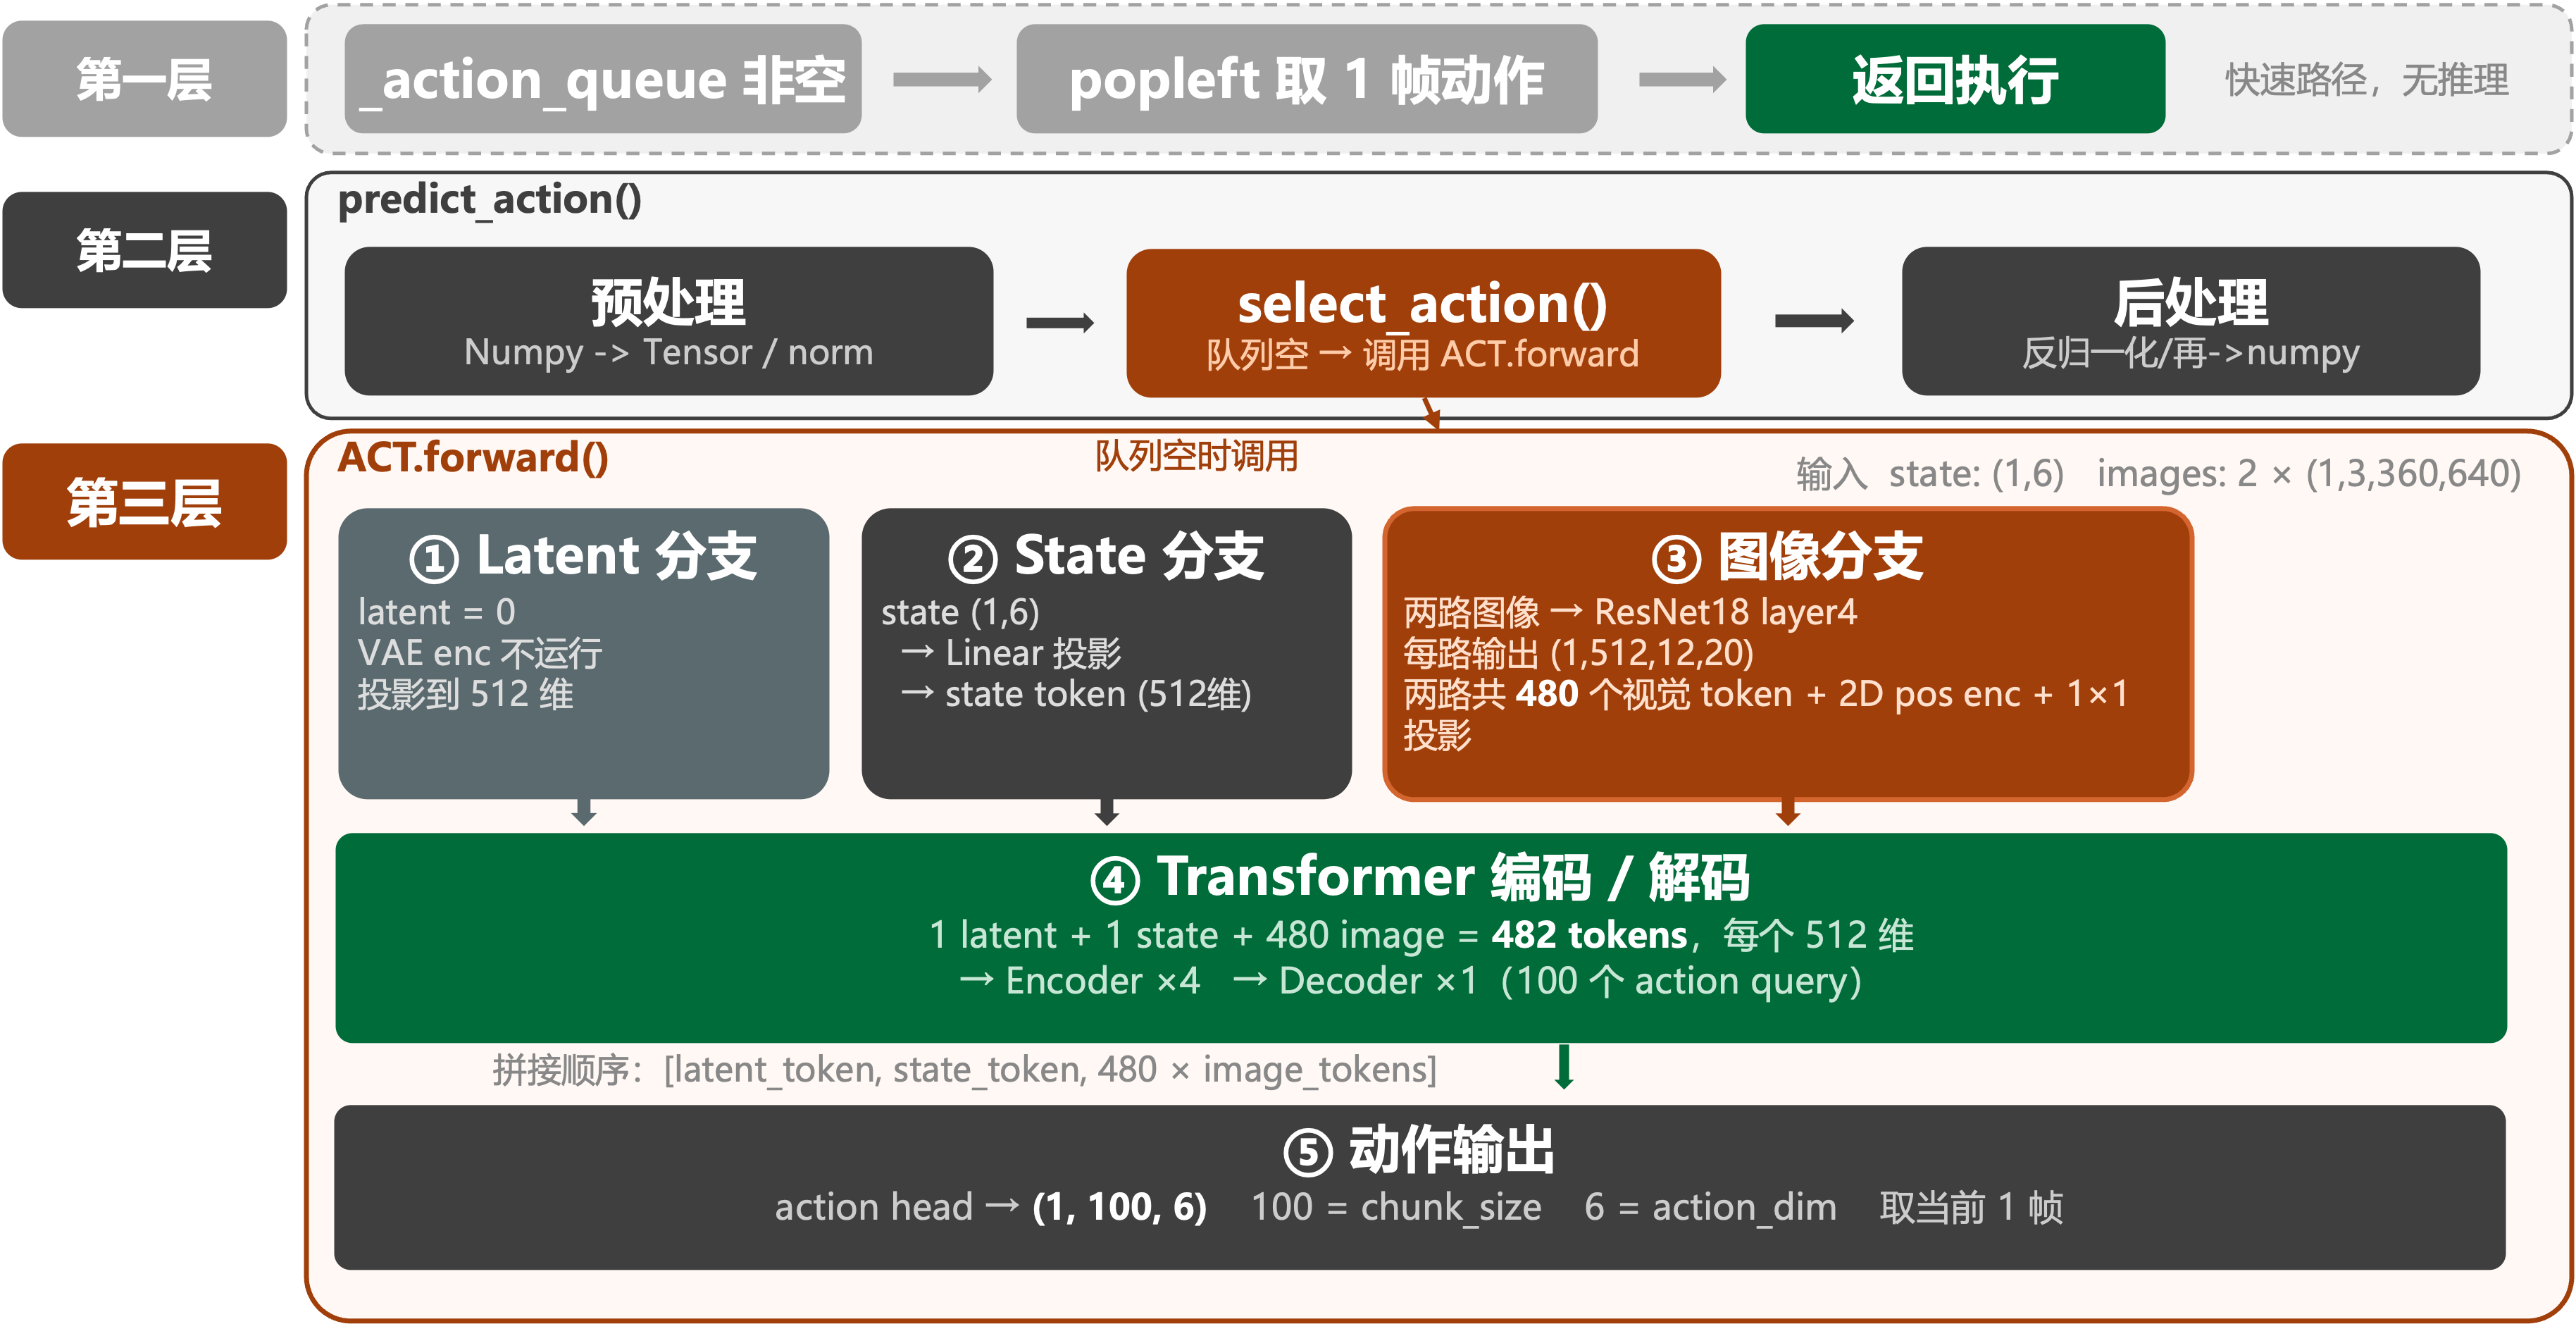
\includegraphics[width=\textwidth]{3_性能分析/image/act_forward_dataflow.png}
  \caption{队列为空时一次完整 ACT 推理的数据流与模型结构}
  \label{fig:act-forward-dataflow}
\end{figure}

其中，视觉分支是主要计算来源。
每路 \(640\times360\) 图像经 ResNet18 的 layer4
得到 \(512\times12\times20\) 特征图，两路相机共形成
480 个视觉 token；再加上 1 个 state token 和 1 个全零 latent token，
构成长度 482、维度 512 的 Transformer Encoder 输入序列。
Decoder 使用 100 个可学习 query，最终通过线性层输出
100 帧、每帧 6 维的归一化动作。

\subsection{chunk\_size 对推理开销分摊与 FPS 的影响}

实验 01 在树莓派 5 上对同一 ACT 抓取瓶子策略扫描 chunk\_size，
取值覆盖 $\{1, 3, 5, 10, 20, 50, 100\}$，每个取值固定记录 20 个 episode，
其它参数（模型权重、分辨率、目标 fps）保持一致。
原始数据与绘图脚本保存在实验 01：chunk\_size 参数扫描中。
后文结合阶段时间占比和 FPS 曲线分析 chunk\_size 对控制循环的影响。

图~\ref{fig:chunk-size-time-pct} 给出了 Observation/Inference/Execution/Wait
（obs/inference/action/wait）四阶段
平均占比（20 episode 均值）随 chunk\_size 变化的曲线。
当 chunk\_size 由 1 增至 100 时，
inference\_pct 从 97.6\% 单调下降到 36.5\%，
对应 wait\_pct 从 0\% 单调上升到 43.3\%；
obs\_pct 从近 0\% 缓慢增长到 15.4\%，
action\_pct 始终保持在 5\% 以内。
这条主曲线说明 chunk\_size 越大，
单帧分摊到的推理工作量就越小，控制循环把更多预算还给等待阶段
（即在帧内等待 fps 节拍），推理不再压满整个 33.3 ms 时间预算。
观测和执行阶段的占比上升只是相对结果——
其绝对耗时基本恒定，只是因为 inference 缩短才在比例上变得显眼。

\begin{figure}[htbp]
  \centering
  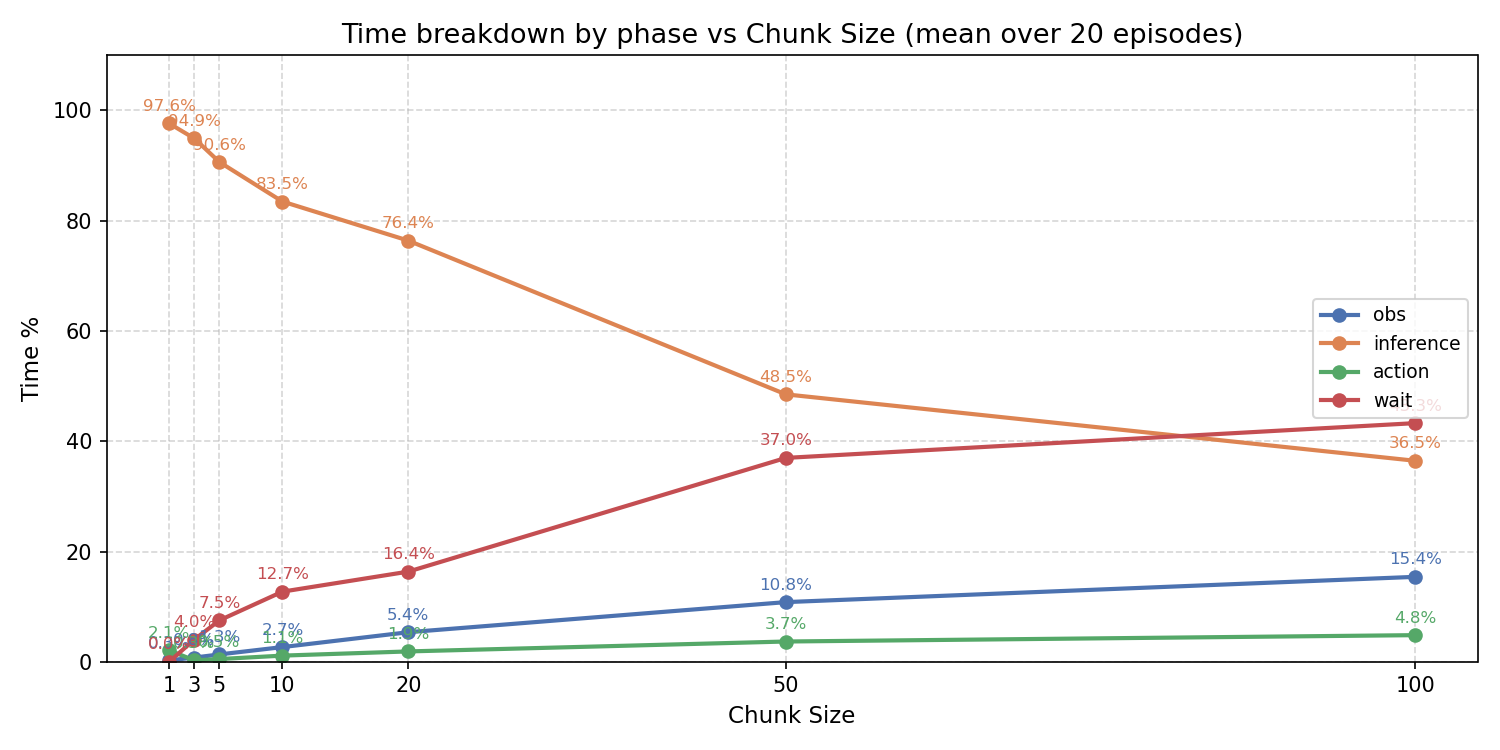
\includegraphics[width=\textwidth]{实验/01_chunk_size参数扫描/chart1_time_pct.png}
  \caption{chunk\_size 对控制循环阶段时间占比的影响}
  \label{fig:chunk-size-time-pct}
\end{figure}

与阶段占比相对应，图~\ref{fig:chunk-size-fps} 给出了实测平均 FPS 随 chunk\_size 的变化曲线。
FPS 在 chunk\_size 从 1 增至 100 的过程中由 0.8 上升到 18.7，
但增长曲线高度非线性：
当 chunk\_size 从 1 增至 10 时，FPS 提升约 6.6 倍（0.8$\to$5.3）；
从 10 增至 50 时再提升约 2.9 倍；
从 50 增至 100 时增益仅约 1.2 倍（15.4$\to$18.7），呈现典型的边际递减。
原因是单次完整 ACT 推理的绝对耗时接近恒定（约 1.5--2.0\,s/次，均值约 1.9\,s），
分块机制只是把这一次重推理在时间上摊薄到更多控制帧上，
而不是降低 ACT 前向计算本身的计算量；
当 chunk\_size 增大到推理被摊薄到接近 fps 目标时，
等待阶段就成为主循环新的瓶颈，进一步增大 chunk\_size 不再带来等比增益。

\begin{figure}[htbp]
  \centering
  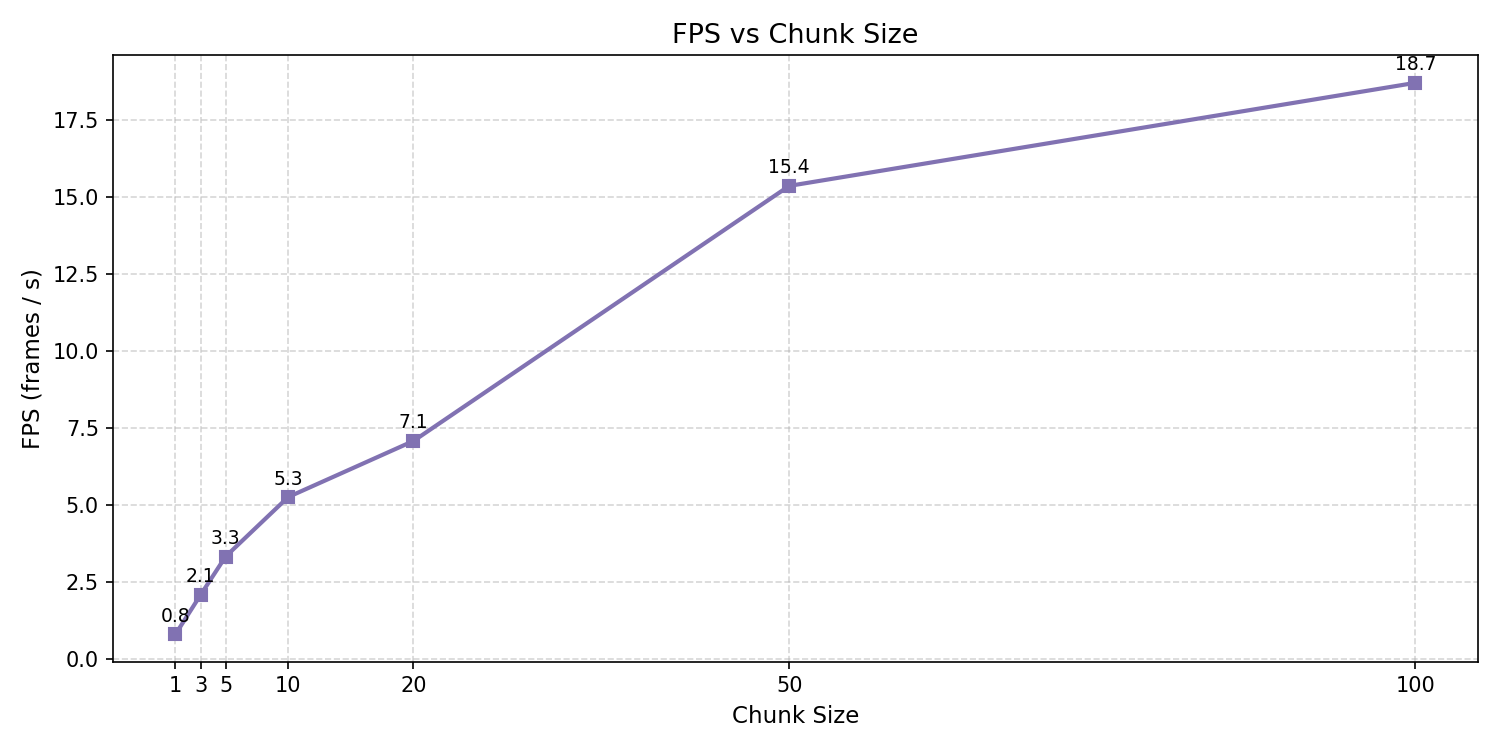
\includegraphics[width=0.92\textwidth]{实验/01_chunk_size参数扫描/chart2_fps.png}
  \caption{chunk\_size 对控制循环 FPS 的影响}
  \label{fig:chunk-size-fps}
\end{figure}


chunk\_size=100 在树莓派 5 上能跑到 $\approx$18.7 fps，距 30 fps 目标仍有约 38\% 缺口；
而此时 wait\_pct 已升至 43.3\%，
说明继续增大 chunk\_size 已经不能进一步把 fps 推到 30——
要逼近目标必须从减小单次推理绝对耗时入手，
也就是后文（第~\ref{ch:opt} 章）讨论的优化方向。

\subsection{单次 ACT 推理耗时分解}\label{sec:act-infer-breakdown}

上面的 episode 级统计能够说明 chunk\_size 如何分摊推理开销，
但还不能回答”一次完整 ACT 推理内部究竟慢在哪里”。
实验在 ACT 模型实现中的动作选择接口和前向计算路径内
插入计时点，通过环境变量 LEROBOT\_PROFILING=1 启用，数据直接写入 CSV。
在树莓派 5 上记录了 6 次队列为空的完整推理，结果汇总于表~\ref{tab:act-single-infer-profile}。

\begin{table}[htbp]
  \centering
  \caption{ACT 单次完整推理（队列为空时）的逐模块耗时分解}
  \label{tab:act-single-infer-profile}
  \small
  \begin{tabular}{lrrr}
  \toprule
  模块 & 平均耗时 ms & 标准差 ms & 占完整推理比例 \\
  \midrule
  动作选择完整路径 & 1924.8 & 414.9 & 100.0\% \\
  \quad ResNet18 + 投影 & 1281.1 & 259.9 & 66.6\% \\
  \quad Transformer Encoder & 569.5 & 506.3 & 29.6\% \\
  \quad Transformer Decoder & 44.0 & 4.4 & 2.3\% \\
  \quad action\_head & 0.7 & 0.8 & $<$0.1\% \\
  队列非空快速路径（对照） & $<$1 ms & — & — \\
  \bottomrule
  \end{tabular}
\end{table}

图~\ref{fig:act-infer-breakdown} 给出了各模块的耗时柱状图。

\begin{figure}[htbp]
  \centering
  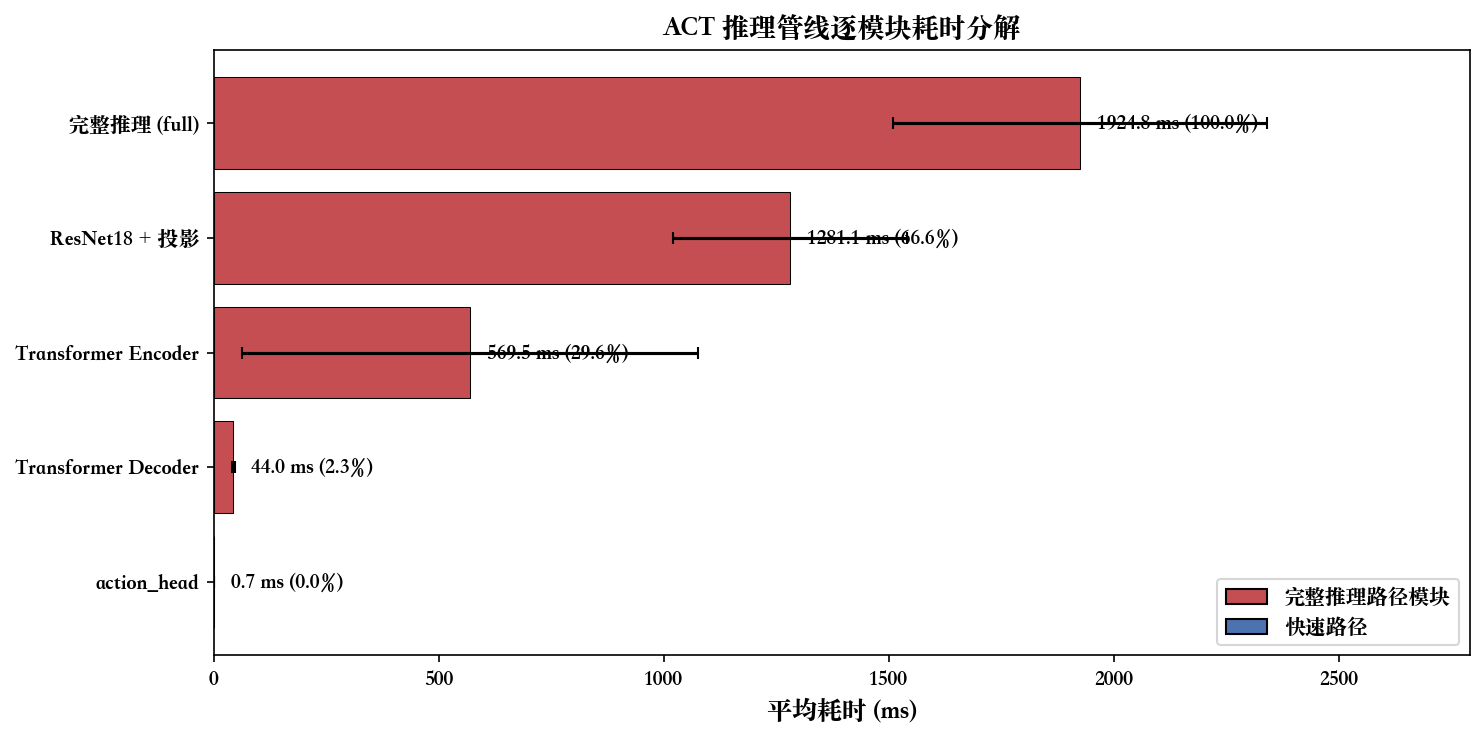
\includegraphics[width=\textwidth]{3_性能分析/image/inference_breakdown.png}
  \caption{ACT 推理管线逐模块耗时分解}
  \label{fig:act-infer-breakdown}
\end{figure}

关键发现：ResNet18 视觉特征提取（两路 ResNet18 backbone + 位置编码 + 1×1 投影）
占据完整推理时间的 66.6\%（平均 1281 ms），是第一瓶颈。
Transformer Encoder 次之，占 29.6\%（569 ms）。
Decoder 和动作输出头占比极低（2.3\% 和 $<$0.1\%），
不是优化重点。
队列非空快速路径耗时不足 1 ms，与后处理相当，
验证了动作缓存机制的有效性。

\subsection{PyTorch 线程行为与推理优化研究现状}\label{sec:thread-behavior}

PyTorch 在 ARM CPU 上使用 OpenMP 并行框架，通过 ATen 线程池调度矩阵运算。
系统调用追踪显示 futex 调用共计 64,569 次 / 40 s episode，
其中 27 线程并行累计等待时间达 3,252 s，
说明多线程同步开销在 ARM CPU 上不可忽略。

推理优化方向（如 INT8 量化、算子融合、线程亲和性、NEON SIMD 加速等）
已有大量文献研究，此处不再展开。
